\documentclass[11pt,a4paper,twocolumn]{article}
\usepackage[english,greek]{babel}
\usepackage[utf8]{inputenc}
\usepackage{nimbusserif}
\usepackage[T1]{fontenc}
\usepackage[left=1.50cm, right=1.50cm, top=2.00cm, bottom=2.00cm]{geometry}
\usepackage{amsmath}
\let\myBbbk\Bbbk
\let\Bbbk\relax
\usepackage[amsbb,subscriptcorrection,zswash,mtpcal,mtphrb,mtpfrak]{mtpro2}
\usepackage{graphicx,multicol,multirow,enumitem,tabularx,mathimatika,gensymb,venndiagram,hhline,longtable,tkz-euclide,fontawesome5,eurosym,tcolorbox,tabularray,pgfplots}
\usetikzlibrary{patterns}
\usepackage[explicit]{titlesec}
\tcbuselibrary{skins,theorems,breakable}
\newlist{rlist}{enumerate}{3}
\setlist[rlist]{itemsep=0mm,label=\roman*.}
\newlist{alist}{enumerate}{3}
\setlist[alist]{itemsep=0mm,label=\alph*.}
\newlist{balist}{enumerate}{3}
\setlist[balist]{itemsep=0mm,label=\bf\alph*.}
\newlist{Alist}{enumerate}{3}
\setlist[Alist]{itemsep=0mm,label=\Alph*.}
\newlist{bAlist}{enumerate}{3}
\setlist[bAlist]{itemsep=0mm,label=\bf\Alph*.}
\newlist{askhseis}{enumerate}{3}
\setlist[askhseis]{label={\Large\thesection}.\arabic*.}
\renewcommand{\textstigma}{\textsigma\texttau}
\newlist{thema}{enumerate}{3}
\setlist[thema]{label=\bf\large{ΘΕΜΑ \textcolor{black}{\Alph*}},itemsep=0mm,leftmargin=0cm,itemindent=18mm}
\newlist{erwthma}{enumerate}{3}
\setlist[erwthma]{label=\bf{\large{\textcolor{black}{\Alph{themai}.\arabic*}}},itemsep=0mm,leftmargin=0.8cm}

\newcommand{\kerkissans}[1]{{\fontfamily{maksf}\selectfont \textbf{#1}}}
\renewcommand{\textdexiakeraia}{}

\usepackage[
backend=biber,
style=alphabetic,
sorting=ynt
]{biblatex}

\DeclareTblrTemplate{caption}{nocaptemplate}{}
\DeclareTblrTemplate{capcont}{nocaptemplate}{}
\DeclareTblrTemplate{contfoot}{nocaptemplate}{}
\NewTblrTheme{mytabletheme}{
\SetTblrTemplate{caption}{nocaptemplate}{}
\SetTblrTemplate{capcont}{nocaptemplate}{}
\SetTblrTemplate{contfoot}{nocaptemplate}{}
}

\NewTblrEnviron{mytblr}
\SetTblrStyle{firsthead}{font=\bfseries}
\SetTblrStyle{firstfoot}{fg=red2}
\SetTblrOuter[mytblr]{theme=mytabletheme}
\SetTblrInner[mytblr]{
rowspec={t{7mm}},columns = {c},
width = 0.85\linewidth,
row{odd} = {bg=red9,fg=black,ht=8mm},
row{even} = {bg=red7,fg=black,ht=8mm},
hlines={white},vlines={white},
row{1} = {bg=red4, fg=white, font=\bfseries\fontfamily{maksf}},rowhead = 1,
hline{2} = {.7mm}, % midrule  
}
\newcounter{askhsh}
\setcounter{askhsh}{1}
\newcommand{\askhsh}{\large\theaskhsh.\ \addtocounter{askhsh}{1}}

\titleformat{\section}{\Large}{\kerkissans{\thesection}}{10pt}{\Large\kerkissans{#1}}

\setlength{\columnsep}{5mm}
\titleformat{\paragraph}
{\large}%
{}{0em}%
{\textcolor{red!80!black}{\faSquare\ \ \kerkissans{\bmath{#1}}}}
\setlength{\parindent}{0pt}

\newcommand{\eng}[1]{\selectlanguage{english}#1\selectlanguage{greek}}

\begin{document}
\twocolumn[{
\centering
\kerkissans{{\huge Τριγωνομετρικές συναρτήσεις}\\\vspace{3mm} {\Large ΑΣΚΗΣΕΙΣ}}\vspace{5mm}}]
\paragraph{Μελέτη συνάρτησης}
\askhsh Για καθεμία από τις παρακάτω συναρτήσεις, να βρεθούν η περίοδος και τα ακρότατα.
\begin{multicols}{2}
\begin{alist}
\item $f(x)=\hm{(3x)}$
\item $f(x)=\syn{(4x)}$
\item $f(x)=\hm{\left(\dfrac{x}{4}\right)}$
\item $f(x)=\syn{\left(\dfrac{x}{3}\right)}$
\item $f(x)=\hm{(\pi x)}$
\item $f(x)=\syn{\left(\dfrac{\pi x}{2}\right)}$
\end{alist}
\end{multicols}
\askhsh Για καθεμία από τις παρακάτω συναρτήσεις, να βρεθούν η περίοδος και τα ακρότατα.
\begin{multicols}{2}
\begin{alist}
\item $f(x)=3\hm{x}$
\item $f(x)=4\syn{x}$
\item $f(x)=\dfrac{\hm{x}}{2}$
\item $f(x)=\dfrac{3\syn{x}}{4}$
\item $f(x)=-3\hm{x}$
\item $f(x)=-2\syn{x}$
\end{alist}
\end{multicols}
\askhsh Για καθεμία από τις παρακάτω συναρτήσεις, να βρεθούν η περίοδος και τα ακρότατα.
\begin{multicols}{2}
\begin{alist}
\item $f(x)=2\hm{(3x)}$
\item $f(x)=2\syn{(4x)}$
\item $f(x)=4\hm{\left(\dfrac{x}{2}\right)}$
\item $f(x)=-2\syn{\left(\dfrac{x}{3}\right)}$
\item $f(x)=-3\hm{(\dfrac{\pi x}{2})}$
\item $f(x)=4\syn{\left(\pi x\right)}$
\end{alist}
\end{multicols}
\askhsh Για καθεμία από τις παρακάτω συναρτήσεις, να βρεθούν η περίοδος και τα ακρότατα.
\begin{alist}
\item $f(x)=2\hm{(2x)}-1$
\item $f(x)=5\syn{(3x)}+3$
\item $f(x)=-3\hm{(3x)}+2$
\item $f(x)=-3\syn{\left(\dfrac{x}{2}\right)}-1$
\item $f(x)=8\hm{(\pi x)}-7$
\item $f(x)=-5\syn{\left(\dfrac{\pi x}{4}\right)}+3$
\end{alist}
\paragraph{Χάραξη γραφικής παράστασης}
\askhsh Δίνεται η συνάρτηση $f(x)=\hm{(2x)}$ με $x\in\mathbb{R}$.
\begin{alist}
\item Να βρεθεί η περίοδος καθώς και τα ακρότατα της $f$.
\item Να χαράξετε τη γραφική παράσταση της $f$ σε διάστημα μιας περιόδου.
\end{alist}
\askhsh Δίνεται η συνάρτηση $f(x)=\syn{(3x)}$ με $x\in\mathbb{R}$.
\begin{alist}
\item Να βρεθεί η περίοδος καθώς και τα ακρότατα της $f$.
\item Να χαράξετε τη γραφική παράσταση της $f$ στο διάστημα $[0,2\pi]$.
\end{alist}
\askhsh Δίνεται η συνάρτηση $f(x)=\syn{\left(\dfrac{x}{2}\right)}$ με $x\in\mathbb{R}$.
\begin{alist}
\item Να βρεθούν η περίοδος και τα ακρότατα της $f$.
\item Να χαράξετε τη γραφική παράσταση της $f$ στο διάστημα $[0,4\pi]$.
\item Βρείτε τα σημεία τομής της $C_f$ με τον άξονα $x'x$.
\end{alist}
\askhsh Δίνεται η συνάρτηση $f(x)=2\hm{x}$ με $x\in\mathbb{R}$.
\begin{alist}
\item Να βρεθούν η περίοδος και τα ακρότατα της $f$.
\item Σχεδιάστε τη γραφική παράσταση της $f$ στο διάστημα $[0,2\pi]$.
\item Βρείτε τα σημεία τομής της $C_f$ με τους άξονες $x'x$ και $y'y$.
\end{alist}
\askhsh Δίνεται η συνάρτηση $f(x)=3\syn{\left(2x\right)}$ με $x\in\mathbb{R}$.
\begin{alist}
\item Να βρεθούν η περίοδος και τα ακρότατα της $f$.
\item Να χαράξετε τη γραφική παράσταση της $f$ στο διάστημα $[0,2\pi]$.
\item Βρείτε τα διαστήματα μονοτονίας της $f$.
\end{alist}
\askhsh Δίνεται η συνάρτηση $f(x)=2\syn{\left(\dfrac{x}{3}\right)}+1$ με $x\in\mathbb{R}$.
\begin{alist}
\item Να βρεθούν η περίοδος και τα ακρότατα της $f$.
\item Να χαράξετε τη γραφική παράσταση της $f$ στο διάστημα $[0,\pi]$.
\item Βρείτε τα διαστήματα μονοτονίας της $f$.
\end{alist}
\askhsh Δίνεται η συνάρτηση $f(x)=3\syn{\left(\pi x\right)}-2$ με $x\in\mathbb{R}$.
\begin{alist}
\item Να βρεθούν η περίοδος και τα ακρότατα της $f$.
\item Να χαράξετε τη γραφική παράσταση της $f$ στο διάστημα $[0,2]$.
\item Βρείτε τα σημεία τομής της $C_f$ με τους άξονες $x'x$ και $y'y$.
\end{alist}
\askhsh Δίνεται η συνάρτηση $f(x)=-2\syn{\left(\dfrac{\pi x}{3}\right)}+3$ με $x\in\mathbb{R}$.
\begin{alist}
\item Να βρεθούν η περίοδος και τα ακρότατα της $f$.
\item Να χαράξετε τη γραφική παράσταση της $f$ στο διάστημα $[0,3]$.
\item Βρείτε τα διαστήματα μονοτονίας της $f$.
\end{alist}


\askhsh Για καθεμία από τις παρακάτω συναρτήσεις, να σχεδιάσετε τη γραφική παράσταση της στο διάστημα $[0,2\pi]$.
\begin{multicols}{2}
\begin{alist}
\item $f(x)=\ef{(2x)}$
\item $f(x)=\syf{(3x)}$
\item $f(x)=\ef{\left(\dfrac{x}{3}\right)}$
\item $f(x)=\syf{\left(\dfrac{x}{2}\right)}$
\end{alist}
\end{multicols}
\askhsh Να χαράξετε στο ίδιο σύστημα συντεταγμένων $x\hat{O}y$ τις γραφικές παραστάσεις των συναρτήσεων $f$ και $g$.
\begin{alist}
\item $f(x)=\hm{x}$ και $g(x)=\hm{(2x)}$
\item $f(x)=\syn{x}$ και $g(x)=\syn{(3x)}$
\item $f(x)=\hm{x}$ και $g(x)=\hm{\left(\dfrac{x}{3}\right)}$
\item $f(x)=\syn{x}$ και $g(x)=\syn{\left(\dfrac{x}{2}\right)}$
\item $f(x)=\hm{x}$ και $g(x)=\hm{(\pi x)}$
\item $f(x)=\syn{x}$ και $g(x)=\syn{\left(\dfrac{\pi x}{2}\right)}$
\end{alist}
\askhsh Να χαράξετε στο ίδιο σύστημα συντεταγμένων $x\hat{O}y$ τις γραφικές παραστάσεις των συναρτήσεων $f$ και $g$.
\begin{alist}
\item $f(x)=\hm{x}$ και $g(x)=2\hm{x}$
\item $f(x)=\syn{x}$ και $g(x)=3\syn{x}$
\item $f(x)=\hm{x}$ και $g(x)=-4\hm{x}$
\item $f(x)=\syn{x}$ και $g(x)=-\dfrac{4\syn{x}}{3}$
\end{alist}
\askhsh Να χαράξετε στο ίδιο σύστημα συντεταγμένων $x\hat{O}y$ τις γραφικές παραστάσεις των συναρτήσεων $f$ και $g$.
\begin{alist}
\item $f(x)=\hm{x}$ και $g(x)=2\hm{(3x)}$
\item $f(x)=\syn{x}$ και $g(x)=4\syn{(2x)}$
\item $f(x)=\hm{x}$ και $g(x)=-3\hm{(4x)}$
\item $f(x)=\syn{x}$ και $g(x)=\dfrac{1}{2}\syn{\left(\dfrac{x}{2}\right)}$
\end{alist}
\askhsh Να χαράξετε στο ίδιο σύστημα συντεταγμένων $x\hat{O}y$ τις γραφικές παραστάσεις των συναρτήσεων $f$ και $g$.
\begin{alist}
\item $f(x)=\ef{x}$ και $g(x)=\ef{(2x)}$
\item $f(x)=\syf{x}$ και $g(x)=\syf{\left(\dfrac{x}{2}\right)}$
\item $f(x)=\ef{x}$ και $g(x)=2\ef{x}$
\item $f(x)=\syf{x}$ και $g(x)=\dfrac{\syf{x}}{2}$
\end{alist}
\askhsh Να χαράξετε στο ίδιο σύστημα συντεταγμένων $x\hat{O}y$ τις γραφικές παραστάσεις των συναρτήσεων $f,g$ και $h$.
\begin{alist}
\item $f(x)=\hm{x},g(x)=\hm{x}+2$ και $h(x)=\hm{x}-1$
\item $f(x)=\syn{x},g(x)=\syn{x}-3$ και $h(x)=\syn{x}+4$
\item $f(x)=\hm{x},g(x)=\hm{(x-\pi)}$ και $h(x)=\hm{\left(x+\dfrac{\pi}{2}\right)}$
\item $f(x)=\syn{x},g(x)=\syn{(x+\pi)}$ και $h(x)=\syn{\left(x-\dfrac{\pi}{2}\right)}$
\end{alist}
\askhsh Να χαράξετε στο ίδιο σύστημα συντεταγμένων $x\hat{O}y$ τις γραφικές παραστάσεις των συναρτήσεων $f$ και $g$.
\begin{alist}
\item $f(x)=\hm{x}$ και $g(x)=2\hm{(3x)}$
\item $f(x)=\syn{x}$ και $g(x)=-3\syn{(2x)}$
\item $f(x)=\hm{x}$ και $g(x)=4\hm{\left(\dfrac{\pi x}{12}\right)}$
\item $f(x)=\syn{x}$ και $g(x)=\dfrac{1}{2}\syn{\left(\dfrac{\pi x}{2}\right)}$
\end{alist}
\paragraph{Άρτιες - Περιττές}
\askhsh Να εξετάσετε αν οι παρακάτω συναρτήσεις είναι άρτιες ή περιττές.
\begin{multicols}{2}
\begin{alist}
\item $f(x)=\dfrac{\hm{x}}{x^2+3}$
\item $f(x)=\dfrac{\hm{x}}{x}$
\item $f(x)=\dfrac{\syn{x}}{|x|-1}$
\item $f(x)=\hm{\left(x^3-x\right)}$
\end{alist}
\end{multicols}
\paragraph{Περιοδικότητα}
\askhsh Να αποδείξετε ότι καθεμία από τις παρακάτω συναρτήσεις είναι περιοδική, με περίοδο τον δοσμένο αριθμό $T$.
\begin{alist}
\item $f(x)=\hm{(2x)}+\syn{(4x)}$, με $T=\pi$
\item $f(x)=\hm{(4x)}+\ef{(2x)}$, με $T=\dfrac{\pi}{2}$
\item $f(x)=\syn{(4x)}+\ef{(4x)}$, με $T=\dfrac{\pi}{2}$
\item $f(x)=\syn{(2x)}\cdot\syf{x}$, με $T=\pi$
\item $f(x)=\syf{(2x)}+\ef{(8x)}$, με $T=\dfrac{\pi}{2}$
\item $f(x)=\hm{(2x)}\cdot\ef{x}$, με $T=\pi$
\item $f(x)=\syn{(3x)}+\ef{(4x)}$, με $T=\dfrac{2\pi}{3}$
\end{alist}
\askhsh
\paragraph{Σύγκριση αριθμών}
\askhsh Να τοποθετήσετε σε αύξουσα σειρά τους παρακάτω τριγωνομετρικούς αριθμούς.
\[ \hm{\left(\dfrac{3\pi}{8}\right)},\hm{\left(\dfrac{\pi}{10}\right)},\hm{\left(\dfrac{\pi}{12}\right)},\hm{\left(\dfrac{5\pi}{12}\right)} \]
\askhsh Να τοποθετήσετε σε αύξουσα σειρά τους παρακάτω τριγωνομετρικούς αριθμούς.
\[ \syn{\left(\dfrac{5\pi}{4}\right)},\hm{\left(\dfrac{7\pi}{6}\right)},\syn{\left(\dfrac{9\pi}{8}\right)},\syn{\left(\dfrac{4\pi}{3}\right)} \]
\askhsh Δίνεται η συνάρτηση $f(x)=2\hm{(4x)}$.
\begin{alist}
\item Να μελετήσετε την $f$ ως προς τη μονοτονία και τα ακρότατα στο διάστημα $\left[0,\frac{\pi}{2}\right]$.
\item Να συγκρίνετε τις τιμές $f\left(\frac{\pi}{3}\right)$ και $f\left(\frac{\pi}{4}\right)$.
\end{alist}
\paragraph{Προβλήματα}
\askhsh Ένα σώμα είναι δεμένο στην άκρη ενός κατακόρυφου ελατηρίου όπως φαίνεται στο σχήμα. Το ύψος, (σε \eng{m}), του σώματος από το έδαφος, κάθε χρονική στιγμή $t$ (σε \eng{sec}), δίνεται από τη συνάρτηση
\begin{center}
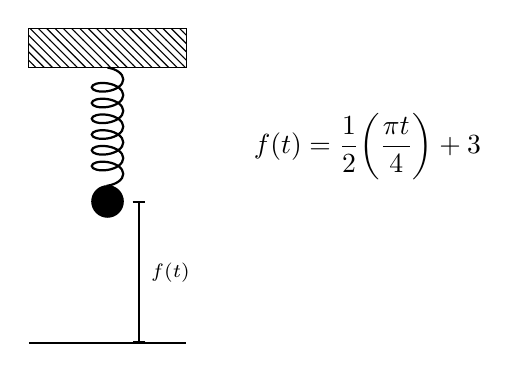
\begin{tikzpicture}
% Wall
\draw[pattern=north west lines] (-1,4) rectangle (1,3.5);
% Spring
\draw[decorate, decoration={coil, segment length=2mm, amplitude=2mm}, thick] (0,3.5) -- (0,2);
% Ball
\draw[fill=black] (0,1.8) circle (0.2cm);
\draw[thick] (-1,0)--(1,0);
\draw[|-|] (0.4,1.8)--(0.4,0.02);
\node at (0.8,0.9) {{\scriptsize $f(t)$}};
\node at (3.3,2.5) {$f(t)=\dfrac{1}{2}\hm{\left(\dfrac{\pi t}{4}\right)}+3$};
\end{tikzpicture}
\end{center}
\begin{alist}
\item Σε τι ύψος βρίσκεται το σώμα όταν το ελατήριο είναι σε κατάσταση ισορροπίας?
\item Πόσα δευτερόλεπτα διαρκεί μια πλήρης ταλάντωση του σώματος?
\item Ποιο είναι το μέγιστο και το ελάχιστο ύψος που μπορεί να φτάσει το σώμα?
\item Βρείτε το χρονικό διάστημα κατά το οποίο το σώμα απομακρύνεται από το έδαφος.
\end{alist}
\askhsh Η θερμοκρασία μιας περιοχής σε βαθμούς κελσίου (°$C$ ) κατά τη διάρκεια ενός εικοσιτετράωρου δίνεται κατά προσέγγιση από τη συνάρτηση:
\[ f(t)=-8\syn{\frac{\pi t}{12}}+4\ ,\ 0\leq t\leq 24 \]
όπου $t$ ο χρόνος σε ώρες.
\begin{alist}
\item Να βρείτε τη μέγιστη και την ελάχιστη θερμοκρασία κατά τη διάρκεια του εικοσιτετράωρου, καθώς και την περίοδο της συνάρτησης.
\item Να παραστήσετε γραφικά την $f$ για $t\in[0,24]$.
\item Να βρείτε με τη βοήθεια της γραφικής παράστασης, σε ποια διαστήματα μέσα στη μέρα η θερμοκρασία αυξάνεται και σε ποια μειώνεται.
\item Να βρείτε, με τη βοήθεια της γραφικής παράστασης, τις ώρες στις οποίες η θερμοκρασία ισούται με $ 8\degree C $.
\end{alist}
\paragraph{Παραμετρικές}
\askhsh Δίνεται η συνάρτηση $f(x)=a\hm{x}, a>0$ η οποία έχει ελάχιστη τιμή το $-2$.
\begin{alist}
\item Να βρεθεί η τιμή της παραμέτρου $a$.
\item Να χαράξετε τη $C_f$ στο διάστημα $[-\pi,2\pi]$.
\end{alist}
\askhsh Δίνεται η συνάρτηση $f(x)=\syn{(\lambda x)}, \lambda>0$ με περίοδο $T=\pi$.
\begin{alist}
\item Να βρεθεί η τιμή της παραμέτρου $\lambda$.
\item Να χαράξετε τη $C_f$ στο διάστημα $[0,2\pi]$.
\end{alist}
\askhsh Δίνεται η συνάρτηση $f(x)=a\hm{(\beta x)}$, με $a,\beta>0$, η οποία έχει περίοδο $T=\pi$ και μέγιστη τιμή $3$.
\begin{alist}
\item Να βρεθούν οι τιμές των παραμέτρων $a$ και $\beta$.
\item Τοποθετήστε τις τιμές $f\left(\frac{\pi}{2}\right),f\left(\frac{\pi}{4}\right)$ και $f\left(\frac{\pi}{3}\right)$ σε φθίνουσα σειρά.
\item 
\end{alist}
\paragraph{Ερωτήσεις θεωρίας}
\askhsh Να χαρακτηρίσετε τις παρακάτω προτάσεις ως σωστές (\textbf{Σωστό}) λανθασμένες (\textbf{Λάθος}).
\begin{alist}
\item Η συνάρτηση $f(x)=\hm{(3x)}$ έχει πεδίο ορισμού το $D_f=\mathbb{R}$.
\item Η συνάρτηση $f(x)=\ef{(2x)}$ έχει πεδίο ορισμού το $D_f=\mathbb{R}$.
\item Οι γραφικές παραστάσεις των συναρτήσεων $f(x)=\hm{x}$ και $g(x)=\syn{\left(\dfrac{\pi}{2}-x\right)}$ ταυτίζονται.
\item Η γραφική παράσταση της συνάρτησης $f(x)=\syn{x}+\dfrac{3}{2}$ τέμνει τον άξονα $x'x$.
\item Η συνάρτηση $f(x)=\syf{x}$ δεν έχει ακρότατα.
\item Η συνάρτηση $f(x)=\ef{x}$ είναι γνησίως αύξουσα στο διάστημα $\left(-\dfrac{\pi}{2},\dfrac{\pi}{2}\right)$.
\item Η συνάρτηση $f(x)=\hm{(4x)}$ είναι περιοδική με περίοδο $T=\dfrac{\pi}{2}$.
\item Η συνάρτηση $f(x)=\ef{(2x)}$ είναι περιοδική με περίοδο $T=\pi$.
\item Η συνάρτηση $f(x)=\hm{(2x)}$ είναι γνησίως φθίνουσα στο διάστημα $\left(\dfrac{\pi}{4},\dfrac{3\pi}{4}\right)$.
\item Οι γραφικές παραστάσεις των συναρτήσεων $f(x)=\syn{x}$ και $g(x)=\syn{(\pi-x)}$ είναι συμμετρικές ως προς τον άξονα $x'x$.
\item Οι γραφικές παραστάσεις των συναρτήσεων $f(x)=\ef{x}$ και $g(x)=\ef{(-x)}$ είναι συμμετρικές ως προς τον άξονα $x'x$.
\end{alist}
\end{document}
